\documentclass[11pt]{utalcaDoc}
\usepackage{alltt}
\usepackage{underscore}
\usepackage[latin1]{inputenc}
\usepackage[activeacute,spanish]{babel}
\usepackage{verbatim}
\usepackage[pdftex]{graphicx}
\usepackage{ae}
\usepackage{amsmath}
\usepackage{amsfonts}
\usepackage{pdflscape}
\usepackage{inconsolata}
\usepackage{url}
\usepackage{listings}
% \usepackage{placeins}
\usepackage[section]{placeins}
\graphicspath{ {images/} }

\title{{\bf Redes de computadoras}\\Informe prelaboratorio}

\author{Erik Regla\\ eregla09@alumnos.utalca.cl}
\date{19 de Abril del 2016}
\lstset{language=SH, 
		basicstyle=\ttfamily\tiny, 
		showspaces=false, 
		numbers=left, 
		breaklines=true,
		frame=shadowbox
		}

\begin{document}
\maketitle

\section{Acercamiento utilizado}
\subsection{Aislamiento}
Subnetting + encapsulaci�n por medio de VLAN
\subsection{Manejo de DHCP}
Asignado como IP helper al router principal.
\subsection{Manejo de DNS}
Asignado al DHCP para propagar su configuraci�n.
\subsection{Switch 8 puertas}
Usado para conectar la mayor�a de la infraestructura de apoyo sobre la VLAN
por defecto. El resto se conecta sobre la VLAN de equipos. Se prefiere
GigabitEthernet para conectar dispositivos para no saturar la red.
\subsection{Switch 24 puertas}
Usado principalmente para conectar pcs de escritorio. Utiliza una GigabitEthernet
para enlazar al router wireless en modo access, para as� poder aislar su subred
bajo la VLAN 3.
\subsection{Manejo de Router Wireless}
Asignado a una VLAN propia aislada del resto. El router inal�mbrico por defecto
NATea las conexiones. Tampoco pueden ver el servidor web (no hay requerimiento
explicitado que los invitados pueden ver el servidor web, por tanto
se obvi�.)
\subsection{Topolog�a}
Basada en MST (Minimum spanning tree) a modo de minimizar los hops entre dispositivos.
\subsection{Equipos} DHCP,DNS,WEB1,WEB2,PRINTER bajo ip fija. Todo el resto mediante DHCP.
\section{Diagramas y configuraci�n de elementos en PacketTracer}

\begin{figure}[!ht]
  \centering
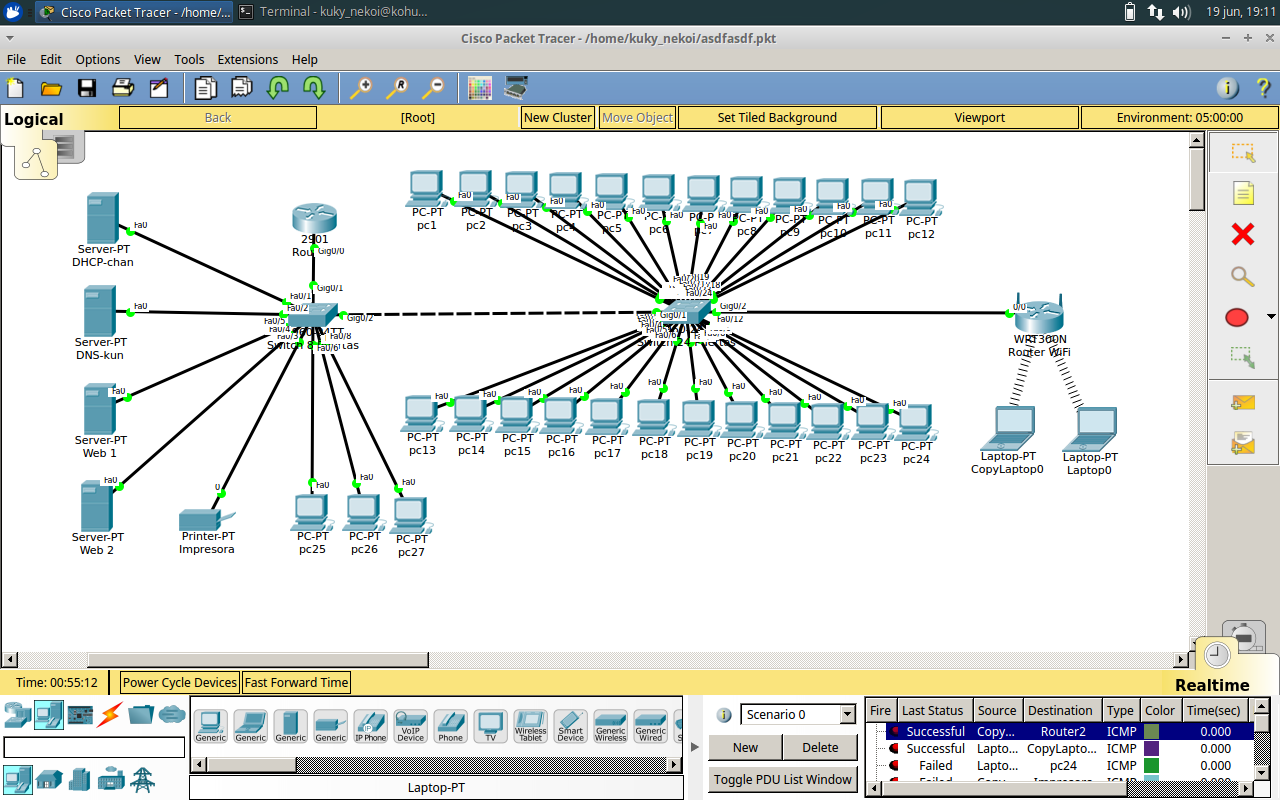
\includegraphics[scale=.3]{pk.png} 
  \caption{Diagrama de PacketTracer}
  \label{FIGURE:MAINDIAGRAM}
\end{figure}

\begin{figure}[!ht]
  \centering
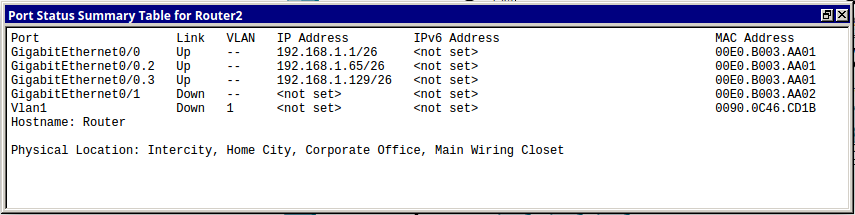
\includegraphics[scale=.3]{router.png} 
  \caption{Listado de puertas Router}
  \label{FIGURE:ROUTER}
\end{figure}

\begin{figure}[!ht]
  \centering
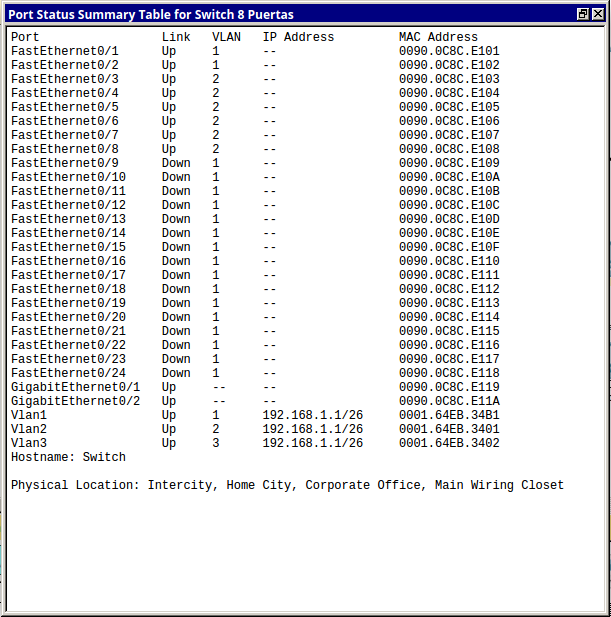
\includegraphics[scale=.3]{switch8.png} 
  \caption{Listado de puertas Switch 8 puertas}
  \label{FIGURE:SWITCH8}
\end{figure}

\begin{figure}[!ht]
  \centering
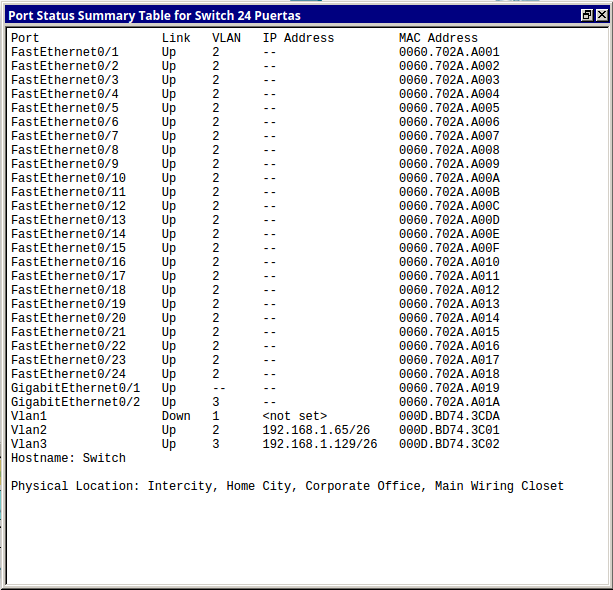
\includegraphics[scale=.3]{switch24.png} 
  \caption{Listado de puertas Switch 24 puertas}
  \label{FIGURE:SWITCH24}
\end{figure}

\begin{figure}[!ht]
  \centering
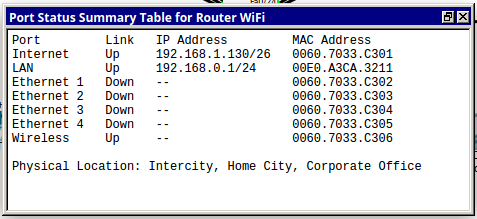
\includegraphics[scale=.3]{wireless.png} 
  \caption{Listado de puertas Router Wireless}
  \label{FIGURE:WIRELESS}
\end{figure}

\begin{figure}[!ht]
  \centering
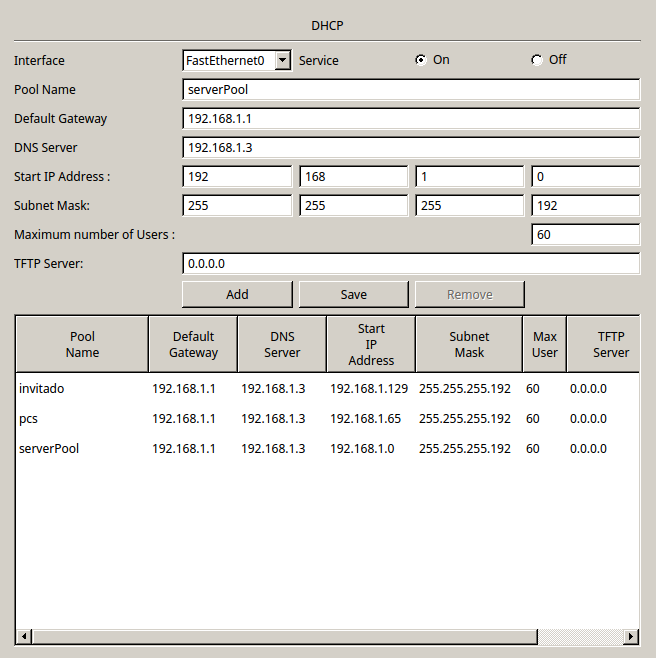
\includegraphics[scale=.3]{dhcp.png} 
  \caption{Configuraci�n DHCP}
  \label{FIGURE:DHCP}
\end{figure}

\begin{figure}[!ht]
  \centering

\includegraphics[scale=.3]{printer.png} 
  \caption{Configuraci�n impresora}
  \label{FIGURE:PRINTER}
\end{figure}


\begin{figure}[!ht]
  \centering

\includegraphics[scale=.3]{printer.png} 
  \caption{Configuraci�n impresora}
  \label{FIGURE:PRINTER}
\end{figure}


\begin{figure}[!ht]
  \centering
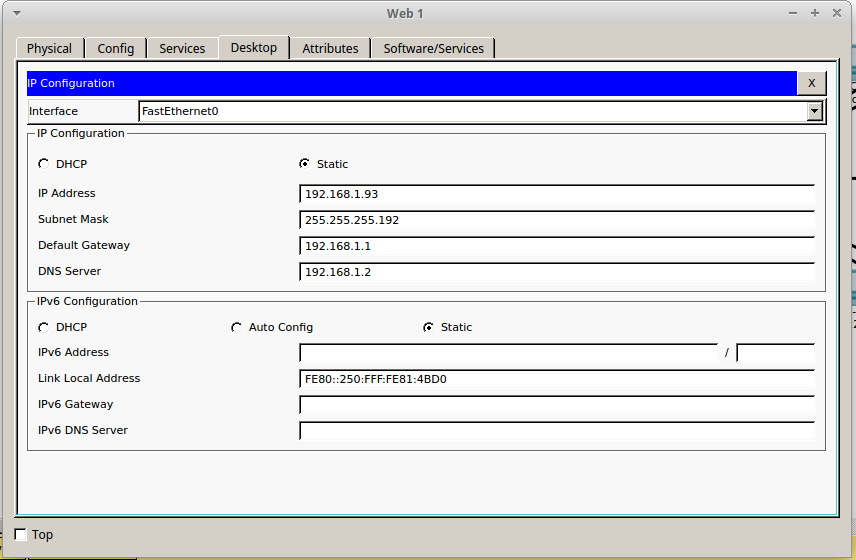
\includegraphics[scale=.3]{web1.png} 
  \caption{Configuraci�n servidor web 1}
  \label{FIGURE:WEB1}
\end{figure}


\begin{figure}[!ht]
  \centering
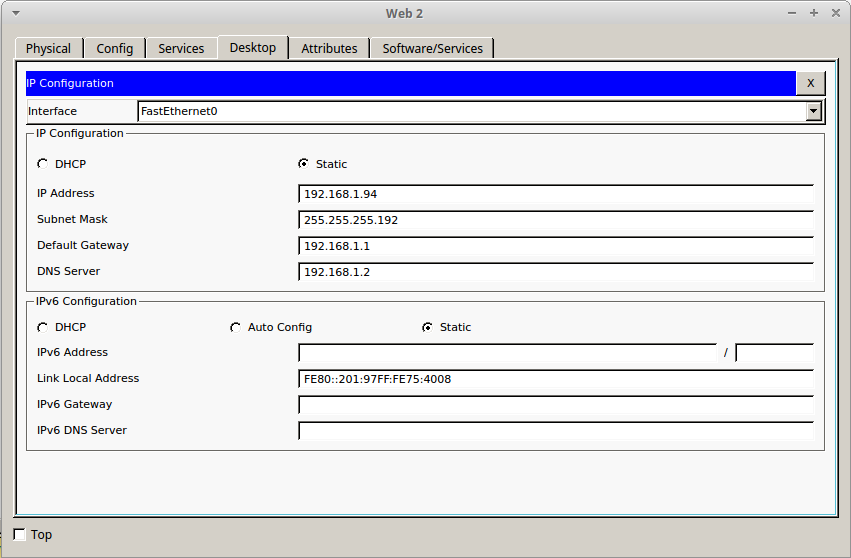
\includegraphics[scale=.3]{web2.png} 
  \caption{Configuraci�n servidor web 2}
  \label{FIGURE:WEB2}
\end{figure}

\section{Calculo de subredes}
\begin{table}[h]
\centering
\caption{Tabla de c�lculo de subredes}
\label{TABLA_SUBREDES}
\begin{tabular}{|c|c|c|c|c|c|c|}
\hline
\textbf{\#} & \textbf{IP Subred} & \textbf{M�scara} & \textbf{Gateway} & \textbf{Broadcast} & \textbf{Rango}                & \textbf{IPs disp.} \\ \hline
0           & 192.168.1.0        & /20              & 192.168.1.1      & 192.168.1.63       & 192.168.1.2 - 192.168.1.62    & 62                       \\ \hline
1           & 192.168.1.64       & /20              & 192.168.1.65     & 192.168.1.127      & 192.168.1.66 - 192.168.1.126  & 62                       \\ \hline
2           & 192.168.1.128      & /20              & 192.168.1.129    & 192.168.1.191      & 192.168.1.130 - 192.168.1.190 & 62                       \\ \hline
3           & 192.168.1.192      & /20              & 192.168.1.193    & 192.168.1.255      & 192.168.1.194 - 192.168.1.254 & 62                       \\ \hline
\end{tabular}
\end{table}

\section{Scripting}

\begin{figure}[!ht]
\begin{lstlisting}
Router#enable
Router#configure terminal
Enter configuration commands, one per line.  End with CNTL/Z.
Router(config)#interface gigabitEthernet 0/0
Router(config-if)#ip address 192.168.1.1 255.255.255.192
Router(config-if)#ip helper-address 192.168.1.2
Router(config-if)#no shutdown 
Router(config-if)#exit
Router(config)#exit
Router>enable
Router#configure terminal
Enter configuration commands, one per line.  End with CNTL/Z.
Router(config)#interface gigabitEthernet 0/0.2
Router(config-subif)#encapsulation dot1Q 2
Router(config-subif)#ip address 192.168.1.65 255.255.255.192
Router(config-subif)#ip helper-address 192.168.1.2
Router(config-subif)#exit
Router(config)#exit
Router#
Router#configure terminal
Enter configuration commands, one per line.  End with CNTL/Z.
Router(config)#interface gigabitEthernet 0/0.3
Router(config-subif)#encapsulation dot1Q 3
Router(config-subif)#ip address 192.168.1.129 255.255.255.192
Router(config-subif)#ip helper-address 192.168.1.2
Router(config-subif)#exit
Router(config)#exit
\end{lstlisting}
\label{FIG:ROUTER}
\caption{Scripting para Router principal}
\end{figure}


\begin{figure}[!ht]
\begin{lstlisting}

Switch>enable
Switch#configure terminal
Switch(config)#vlan 1
Switch(config-vlan)#name admin
Switch(config-vlan)#exit
Switch(config)#vlan 2
Switch(config-vlan)#name pc
Switch(config-vlan)#exit
Switch(config)#vlan 3
Switch(config-vlan)#name invitado
Switch(config-vlan)#exit
Switch(config)#interface range fastEthernet 0/1-2
Switch(config-if-range)#switchport access vlan 1
Switch(config-if-range)#exit
Switch(config)#interface range fastEthernet 0/3-8
Switch(config-if-range)#switchport access vlan 2
Switch(config-if-range)#exit
Switch(config)#no shutdown
Switch(config)#interface range fastEthernet 0/6-8
Switch(config-if-range)#no shutdown
Switch(config-if-range)#exit
Switch(config)#interface range fastEthernet 0/1-5
Switch(config-if-range)#no shutdown
Switch(config-if-range)#exit
Switch(config)#interface vlan 1
Switch(config-if)#ip address 192.168.1.1 255.255.255.192
Switch(config-if)#no shutdown
Switch(config-if)#exit
Switch(config)#interface vlan 2
Switch(config-if)#ip address 192.168.1.1 255.255.255.192
Switch(config-if)#no shutdown
Switch(config-if)#exit
Switch(config)#interface vlan 3
Switch(config-if)#ip address 192.168.1.1 255.255.255.192
Switch(config-if)#no shutdown
Switch(config-if)#exit
Switch(config)#interface GigabitEthernet 0/1
Switch(config-if)#switchport mode trunk
Switch(config-if)#exit
Switch(config)#interface range GigabitEthernet 0/1-2
Switch(config-if)#switchport mode trunk
Switch(config-if)#exit
Switch(config)#exit
Switch#copy running-config startup-config 
Destination filename [startup-config]? 
Building configuration...
[OK]
\end{lstlisting}
\label{FIG:SWITCH8}
\caption{Scripting para Switch 8 puertas}
\end{figure}

\begin{figure}[!ht]
\begin{lstlisting}
Switch>enable
Switch#configure terminal
Enter configuration commands, one per line.  End with CNTL/Z.
Switch(config)#vlan 2
Switch(config-vlan)#name pc
Switch(config-vlan)#exit
Switch(config)#vlan 3
Switch(config-vlan)#name invitado
Switch(config-vlan)#exit
Switch(config)#interface range fastEthernet 0/1-24
Switch(config-if-range)#switchport access vlan 2
Switch(config-if-range)#no shutdown
Switch(config-if-range)#exit
Switch(config)#interface vlan 2
Switch(config-if)#ip address 192.168.1.65 255.255.255.192
Switch(config-if)#no shutdown
Switch(config-if)#exit
Switch(config)#interface vlan 3
Switch(config-if)#ip address 192.168.1.129 255.255.255.192
Switch(config-if)#no shutdown
Switch(config-if)#exit
Switch(config)#interface range GigabitEthernet 0/1-2
Switch(config-if)#switchport mode trunk
Switch(config-if)#exit
Switch(config)#interface GigabitEthernet 0/2
Switch(config-if)#switchport access vlan 3
Switch(config-if)#no shutdown
Switch(config-if)#exit
Switch(config)#exit
Switch#copy running-config startup-config
\end{lstlisting}
\label{FIG:SWITCH24}
\caption{Scripting para Switch 8 puertas}
\end{figure}



\end{document}
